\documentclass{mgragh} % opcje: robocza,man
\usepackage[cp1250]{inputenc}  % opcja latin2 dla Linuxa lub cp1250 dla Windows
\usepackage[polish]{babel}
\usepackage[OT4]{fontenc}
\usepackage{polski}
\usepackage{graphicx}

%%
%%
\makeindex 
% \includeonly{Mgr_pom,Mgr_wst,Mgr_roz1,Mgr_roz2,Mgr_lit}

%\bibliographystyle{ddabbrv}
\bibliographystyle{bibtex}
%\nocite{*}

\begin{document}
%%
%%
%% ======== METRYCZKA PRACY ========
\title{Komponentowa architektura indukcyjnej bazy danych jako platformy uczenia
maszynowego}
\author{Nikodem Jura, Krzysztof Rajda}
\promotor{dr hab. in�. Marek Kisiel-Dorohinicki}
\nralbumu{11957}
\uczelniaNazwa{Akademia G�rniczo-Hutnicza}
\uczelniaImienia{im. Stanis�awa Staszica}
\wydzial{Elektroniki, Automatyki, Informatyki i Elektrotechniki}
\kierunek{Informatyka}
\specjalnosc{In�ynieria system�w informatycznych i baz danych}
\rok{2006}

\maketitle
%%
\slowakluczowe{}

%\keywords{a,b,c,d,e,f,g,h} 
%%
%%
%% ======== NASZE MAKRA ========
%%

%----------------- nasze definicje -----------------% 
\newtheorem{stw}{\indent Stwierdzenie}[chapter]
%------------------------------%
\newcommand{\id}[1]{\index{#1}}  
\newcommand{\wi}[1]{#1\index{#1}}  
\newcommand{\wwi}[1]{\emph{#1}\index{#1}}  
\newcommand{\mwi}[1]{\textbf{#1}\index{#1}}
\newcommand{\ii}[1]{\textit{#1}}
%\newcommand{}{}

%---------------------------------------------------%



%%
%% ======== SPIS TRE�CI ========
%%
\tableofcontents
%%
%% ======== STRESZCZENIE PRACY (POLSKIE) ========
\begin{streszczenie}
%%

%--------------------------------------------------------------------%

%%
\end{streszczenie}
%%
%% ======== G��WNA CZʌ� PRACY ========
%%
%% ==== WST�P ====
%%
\begin{wstep}
%%
\section{Wprowadzenie}
%\subsection{Machine learning}
%\subsection{Indukcyjne bazy danych}
%\subsection{Zastosowania}

Integracja technologii baz danych z nowoczesnymi metodami indukcyjnego
generowania wiedzy wydaje si� dawa� istotne korzy�ci w perspektywie
budowy system�w wspomaganie decyzji. Systemy nazywane czasem
indukcyjnymi bazami danych potrafi� odpowiedzie� nie tylko na pytania,
dla kt�rych odpowied� znajduje si� w bazie danych, ale r�wnie� na
pytania, kt�re wymagaj� zsyntetyzowania i zastosowania wiarygodnej
wiedzy, wygenerowanej przez indukcyjne wnioskowanie z fakt�w z bazy
danych i wcze�niejszej wiedzy.  Indukcyjne bazy danych mog� by�
postrzegane jako naturalny krok w rozwoju system�w bazodanowych \cite{bib3}.

\begin{figure}[ht]
    \centering
        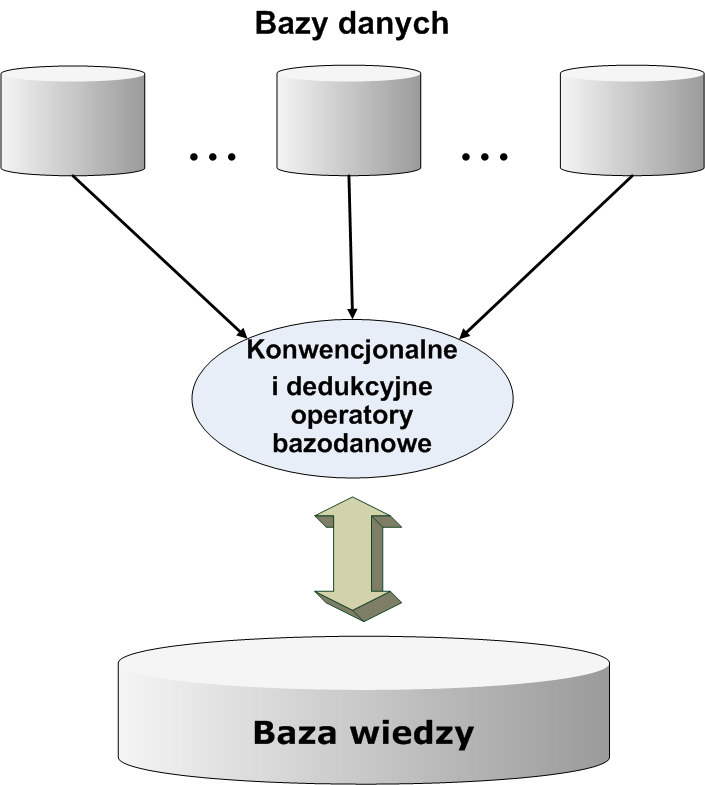
\includegraphics[width=0.70\textwidth]{img/knowledge_mining.png}
    \caption{Indukcyjne bazdy danych}
    \label{fig:architecture}
\end{figure}

\bigskip
W pracy przedstawiona zostanie architektura i wybrane aspekty
implementacji platformy \emph{Salomon}, jak r�wnie� zaprezentowane
zostan� mo�liwo�ci jego wykorzystania na przyk�adzie wybranych
algorytm�w pozyskiwania wiedzy z danych.

%\newpage
%%
\end{wstep}
%%
%% ==== ROZDZIA� 1 ====
%%
%% A tutaj tak dla przyk�adu jest \part
\part{Wprowadzenie}

\chapter{Indukcyjne bazy danych}
%%
\section{Indukcyjne bazy danych}

% przetlumaczone z~pdf-a
Indukcyjne bazy danych �ci�le integruj� bazy danych z~koncepcj� \emph{data mining}~(\ref{lab:data_mining}).
G��wn� ich ide� stanowi to, �e zar�wno dane jak i~wzorce s� przetwarzane 
w ten sam spos�b, a~indukcyjny j�zyk zapyta� pozwala u�ytkownikowi 
na zadawanie zapyta� i~manipulacj� danymi wzorcami.

Od pocz�tku istnienia idei data miningu zdawano sobie spraw�,
�e proces ich przetwarzania powinien by� wspierany przez technologi� baz danych.
W ostatnich latach idea ta zosta�a sformalizowana jako koncepcja
\emph{indukcyjnych baz danych}.

%cytat z~artykulu
Integracja technologii baz danych z~nowoczesnymi metodami
indukcyjnego generowania wiedzy jest naturalnym kierunkiem rozwoju
system�w bazodanowych. Systemy nazywane indukcyjnymi bazami
danych potrafi� odpowiedzie� nie tylko na pytania, dla kt�rych
odpowied� znajduje si� w~bazie danych, ale r�wnie� na pytania,
kt�re wymagaj� zsyntetyzowania i~zastosowania wiedzy,
wygenerowanej przez indukcyjne wnioskowanie z~fakt�w z~bazy danych
i wcze�niejszej wiedzy~\cite{knowledge_disc}. Schemat typowej indukcyjnej
bazy danych przedstawiony jest na rysunku~\ref{fig:inddb}.

\begin{figure}[!ht]
     \centering
         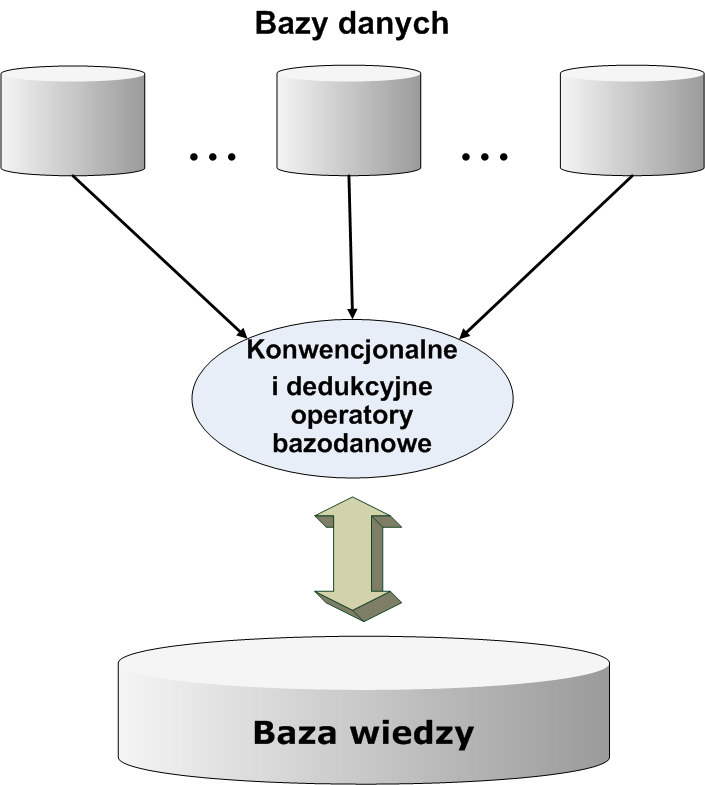
\includegraphics[width=0.90\textwidth]{img/knowledge_mining.png}
     \caption{Indukcyjna baza danych~\cite{ind_databases}}
     \label{fig:inddb}
\end{figure}

Jak zosta�o ju� wy�ej wspomniane, indukcyjne bazy danych przechowuj� nie dane
ale r�wnie� wzorce. Mo�na za�o�y�, �e zar�wno dane, jak i~wzorce stanowi� zbiory zbior�w.
To za�o�enie wynika z~analogii do tradycyjnych, relacyjnych baz danych. 
Relacyjna baza danych zawiera zbi�r relacji, kt�re to~stanowi� zbiory \emph{tupli}, 
a wi�c mo�na powiedzie�, ze stanowi zbi�r zbior�w.

W przypadku baz indukcyjnych rozr�nia si� natomiast zbi�r trenuj�cy od testuj�cego, 
zbi�r poprawnie zaklasyfikowanych przyk�ad�w od zaklasyfikowanych b��dnie itp.
 
To samo, co tyczy si� danych, odnosi si� r�wnie� do wzorc�w.
I rzeczywi�cie -- podczas procesu przetwarzania wiedzy mo�na pracowa� 
na r�nych zbiorach wzorc�w.  Zbiory te mog� odnosi� si� do odmiennych hipotez 
stworzonych na podstawie r�nych zbior�w danych,
czy r�nych ustawie� parametr�w algorytm�w je tworz�cych.

%jezyk (z pdf-a)
Jednym z~zasadniczych powod�w, kt�re przyczyni�y si� do sukcesu relacyjnych baz danych
jest opracowanie uniwersalnego j�zyka zapyta�, kt�ry podobnie jak sama algebra relacyjna
dostarcza du�ych mo�liwo�ci przy jego relatywnej prostocie.

Podobnymi cechami powinien wyr�nia� si� j�zyk zapyta� do indukcyjnych baz danych.

Rezultatem zapytania wykonanego w~takim j�zyku jest albo zbi�r wzorc�w, albo zbi�r danych.
Jest to~tak zwana \emph{w�asno�� zamkni�cia} (\emph{ ang. closure property}).
Stanowi ona analogi� do rezultat�w zapytania do relacyjnych baz danych, gdzie jest nim zawsze relacja.
Rozr�nianie mi�dzy zbiorami wzorc�w i~zbiorami danych powoduje, �e potrzebne s� dwa rodzaje zapyta�:
te kt�re generuj� zbiory wzorc�w i~zbiory danych. Zapytania do jednocze�nie obu typ�w zbior�w nazywane
s� czasami \emph{zapytaniami krzy�uj�cymi} (\emph{ang. cross-over operations}).

%dodawanie/usuwanie data setow, patternow? (patternow trudniej, nie wiem dokladnie jak, olac na razie)

%wnioskowanie
% z~pdf-a
Teoria indukcyjnych baz danych mo�e by� u�yteczna tylko w~przypadku,
gdy oferuje mo�liwo�� wnioskowania z~danych i~zgromadzonej wiedzy.
Na podstawie otrzymanej informacji trenuj�cej indukcyjna baza danych generuje now� lub 
ulepsza wcze�niej posiadan� wiedz�, w~pewien ustalony spos�b reprezentowan� 
i przeznaczon� do wykorzystania przy wykonywaniu okre�lonego zadania.
Mechanizm, zgodnie z~kt�rym dokonuje si� nabywanie lub doskonalenie wiedzy, 
jest najcz�ciej jednoznacznie wyznaczany przez metod� reprezentacji 
wiedzy oraz posta� informacji trenuj�cej \cite{ind_databases}.

\subsection{VINLEN}
\label{lab:vinlen}
Vinlen  \cite{vinlen} to system indukcyjnej bazy danych, rozwijany w
\emph{George Mason University}. Jest to~klasyczna
realizacja indukcyjnej bazy danych. Mechanizmy wnioskowania
indukcyjnego s� zintegrowane ze standardowymi relacyjnymi
operatorami bazodanowymi. Integracja ta opiera si� na nowych
rodzajach operator�w zwanych operatorami generowania wiedzy
\emph{KGO} (Knowledge Generation Operators). \emph{KGO} operuje na
\emph{segmentach wiedzy} sk�adaj�cych si� z~kombinacji jednej lub
wi�cej tabel z~relacyjnej bazy danych i~wiedzy przechowywanej
w~bazie wiedzy (por. rysunek~\ref{fig:inddb}). \emph{KGO} przyjmuje
na wyj�ciu jeden lub wi�cej segment wiedzy, na podstawie kt�rego
generuje inny segment wiedzy. Podstawowym operatorem u�ywanym w
systemie jest AQ21, program do indukcyjnego tworzenia regu� na
podstawie danych.

Indukcyjne bazy danych mog� by� wspierane przez wyspecjalizowanych
agent�w (\emph{Scauts}), kt�rych zadaniem jest synteza
i~zarz�dzanie wiedz�, kt�ra jest dostosowywana do wymaga�
okre�lonego u�ytkownika. System \emph{VINLEN} pozwala na tworzenie skrypt�w
operuj�cych na bazach danych, wiedzy i~algorytmach uczenia
maszynowego przy u�yciu j�zyka \emph{KGL-1} (\emph{Knowledge
Generation Language}).

Cech� charakterystyczn� tak rozwijanego systemu b�dzie mo�liwo��
sk�adowania wiedzy w~relacyjnej bazie danych wraz z~danymi,
zadawanie zapyta� oraz manipulowanie wiedz� z~wykorzystaniem
j�zyka \emph{KQL} lub przy u�yciu funkcjonalnego, graficznego
interfejsu u�ytkownika.


%%
\mgrclosechapter
%%
%% ==== ROZDZIA� 2 ====
%%
% \input{Mgr_roz2}
%%
%%
%% ======== DODATKI ========
%%
%%
%% ======== BIBLIOGRAFIA ========
%%
\newpage

\begin{thebibliography}{99}
\bibitem {bib2} {Kaufman, K. and Michalski, R.S., The Development
    of the Inductive Database System VINLEN: A Review of Current
    Research, International Intelligent Information Processing and
    Web Mining Conference, Zakopane, Poland, 2003}

\bibitem {bib3} {Michalski, R.S. and Kaufman, K., Data Mining and
    Knowledge Discovery: A Review of Issues and a Multistrategy
    Approach, Machine Learning and Data Mining: Methods and
    Applications, R. S. Michalski, I. Bratko and M.  Kubat (Eds.), pp.
    71-112, London: John Wiley \& Sons, 1998}

\bibitem {bib4} {Michalski, R.S., Knowledge Mining and Inductive
    Databases: An Emerging New Research Direction, School of
    Computational Sciences, George Mason University, 2004}

\bibitem {yale} {Mierswa, I., Klinkenberg, R., Fischer, S., Ritthoff, O.,
    A Flexible Platform for Knowledge Discovery Experiments:
    YALE -- Yet Another Learning Environment,
    LLWA 03 - Tagungsband der GI-Workshop-Woche Lernen - Lehren - Wissen -
    Adaptivit�t, 2003.}

\bibitem{uci} {Newman, D.J., Hettich, S., Blake, C.L., Merz, C.J.,
UCI Repository of machine learning databases, Irvine, CA, 1998.}

\bibitem {weka} {Witten, I.H., Frank, E., Data Mining: Practical Machine Learning Tools and
Techniques, Morgan Kaufmann, 2005}



\end{thebibliography}

%%
%% ======== DODATKOWE ELEMENTY PRACY (nieobowi�zkowe) ======== 
%%
%\printindex  
%%

\end{document}